\documentclass[11pt]{standalone}

\usepackage{pgfplots}
\usetikzlibrary{hobby}
\pgfplotsset{compat=newest}

\begin{document}
	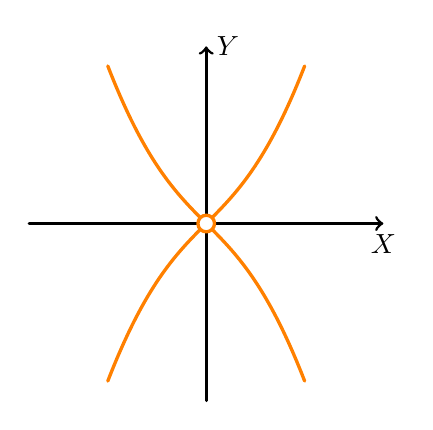
\begin{tikzpicture}[line cap=round, line join=round]
	\draw[->, line width=1] (-2.25,0) -- (2.25, 0) node[below] {$X$};
	\draw[->, line width=1] (0,-2.25) -- (0,2.25) node[right] {$Y$};
	\draw[domain=-1.25:1.25,variable=\x, orange, line width=1.2] plot[quick hobby] (\x, {\x *sqrt(\x*\x +1)});
	\draw[domain=-1.25:1.25,variable=\x, orange, line width=1.2] plot[quick hobby] (\x, {-\x *sqrt(\x*\x +1)});
	\draw[orange, fill=white, line width=1.2pt] (0,0) circle (3pt);
	\end{tikzpicture}
\end{document}